\documentclass[10pt]{article}
\usepackage[OT1]{fontenc}
\usepackage[utf8]{inputenc}
\bibliographystyle{plain}

\usepackage{algorithm2e}
\usepackage{amsmath}
\usepackage{amssymb}
\usepackage{gensymb}
\usepackage{mathrsfs}
\usepackage{mathtools}
\usepackage{esint}
\usepackage{braket}
\usepackage{array}
\usepackage{epsfig}
\usepackage{hyperref}
\renewcommand{\baselinestretch}{1.2}
\setlength{\textheight}{9in}
\setlength{\textwidth}{6.5in}
\setlength{\headheight}{0in}
\setlength{\headsep}{0in}
\setlength{\topmargin}{0in}
\setlength{\oddsidemargin}{0in}
\setlength{\evensidemargin}{0in}
\setlength{\parindent}{.3in}


\DeclarePairedDelimiter{\abs}{\lvert}{\rvert} %create the norm sign as symbol
\DeclarePairedDelimiter{\norm}{\lVert}{\rVert} %create the norm sign as symbol

% swap definition of \abs* and \norm* with \abs and \norm
% to scale delimiters without needing to type *
\makeatletter
\let\oldabs\abs
\def\abs{\@ifstar{\oldabs}{\oldabs*}}
\let\oldnorm\norm
\def\norm{\@ifstar{\oldnorm}{\oldnorm*}}
\makeatother

%custom commands here
% \newcommand{\new_command_name}{replacement text}


\begin{document}
\begin{center}
    \textbf{\large Beyond mean field solutions to the lattice mixture model} \\
    Gabriel Brown
\end{center}

%OUTLINE
% statistical thermodynamics review?
% lattice model
% - coordination number, dimension
% - energy of interaction
% - simple results and equations
% - mean field approximation and internal energy formula
% computational approach
% some extremum bounds
%

\section{Lattice model of a mixture} \footnote{The present description of a mixture on a lattice follows closely to \cite{dill}, with minor modifications and my own motivations and explanations.} 
\subsection{Basics}
A mixture of two condensed (liquid or solid) phases $A$ and $B$ may be crudely described by a single-degree-of-freedom-per-site lattice model with uniform coordination number $z$, meaning that each lattice site has $z$ nearest neighbors.
Restricting the energetic interactions to nearest neighbor pairwise, there are three energetic constants for $A-A$, $B-B$, and $A-B$ interactions, respectively: $w_{AA}, \; w_{BB}, \; w_{AB}$, which may be generically positive, negative, or zero.
Let $W$ represent a realization or configuration of the lattice, uniquely specifying the occupation of each site as $A$ or $B$.
The total internal energy $U$ of such a configuration is then given by
\begin{align}
    U(W) = m_{AA} w_{AA} + m_{BB} w_{BB} + m_{AB} w_{AB}
\end{align}
where $m_{XY}$ is the number of $X-Y$ interactions in the system.
Restricting to finite periodic lattice of $N$ total sites with $N_A$ $A$ sites and $N_B$ $B$ sites (uniquely defining a $B$ volume fraction $x = N_B / N$), one can further define the $m_{XY}$s.
Since each pairwise interaction involved two sites, the total number of interactions for a periodic lattice with $N$ sites and coordination $z$ is
\begin{align}
    m_{AA} + m_{BB} + m_{AB} = \frac{z N}{2} = \frac{z}{2} \left( N_A + N_B \right),
\end{align}
further,
\begin{align}
    \frac{z N_A}{2} = m_{AA} + \frac{m_{AB}}{2}, \quad\quad
    \frac{z N_B}{2} = m_{BB} + \frac{m_{AB}}{2}.
\end{align}
With $N$ and $x=N_B/N$ (equivalently $N_A$ and $N_B$) being known system constants, this model is nearly analytical apart from the unknown value of $m_AB$. \footnote{Realistic physical systems are often so large that it is more convenient to work in terms of densities like $N/V$, but since we will be interacting intimately with the lattice description, we maintain use of $N$ directly.} \footnote{One could also treat $m_{AA}$ or $m_{BB}$ as unknowns, the three $m_{\cdot}$ are algebraically related sucht that one of the three uniquely defines the others.}

\section{Computational Implementation}
discuss Metropolis Monte Carlo algorithm (cite MD book)

discuss energy decomposition trick to make each update step

discuss relaxation scheme

discuss forcing every step to exchange A and B

discuss convergence tolerance


\subsection{Approximate solution}
To keep such a lattice model analytical, we use the Bragg-Williams mean field approximation, which posits that the $A$ and $B$ sites are randomly distributed throughout the lattice.
One can then approximate that $A$ sites have on average $z N_B / N$ neighboring $B$ sites, and the corresponding approximation for $m_{AB}$ is
\begin{equation}
    m_{AB} \approx \frac{z N_A N_B}{N} = z N (1-x) x.
\end{equation}
The standard way of writing the total energy of this model is
\begin{align}
    U &=
    \frac{z w_{AA}}{2} N_A +
    \frac{z w_{BB}}{2} N_B +
    k_B T \chi_{AB} \frac{N_A N_B}{N}, \\
    \chi_{AB} &=
    \frac{z}{k_B T} \left( w_{AB} - \frac{w_{AA} + w_{BB}}{2} \right)
\end{align}
where $\chi_{AB}$ is the dimensionless ``exchange parameter''. \footnote{Admittedly, I don't see the utility in artificially introducing temperature dependence to a temperature-independent model via $\chi_{AB}$, but I believe the dimensionless parameter does have some merit for extracting properties from experiment.}
The formula for average energy $\hat{U}=U/N$ per site is then
\begin{align}
    \hat{U} &=
    \frac{z w_{AA}}{2} (1-x) +
    \frac{z w_{BB}}{2} x +
    k_B T \chi_{AB} (1-x) x
\end{align}
which is useful for working with lattices of varying sizes.

We finish the introduction of the lattice model and mean field approximation by noting how the possible errors associated with the Bragg-Williams approximation, which will require a bit of statistical thermodynamics.
The internal energy of a system in a given macrostate (in this case given by system size $N$ and $B$ volume fraction $x$) generically depends on the energies of all the possible microstates $W_i$. \footnote{As an example, for a 1-D system of a binary mixture of macrostate $N=3$ and $x=1/3$ the possible microstates are $[A,A,B],\; [A,B,A],\; [B,A,A]$. In this case, all microstates have the energy, but it should be clear that for larger systems this will generally not be the case.}
Specifically, the energy of a macrostate is given by
\begin{align}
    U = \sum_{i=1}^{N_{micro}} p_i E_i
    = \frac{1}{Q} \sum_{i=1}^{N_{micro}} E_i \exp\left(\frac{-E_i}{k_B T}\right)
\end{align}
where the sum runs over all possible microstates of the macrostate, and $k_B$ is the Boltzmann constant ($8.617 \times 10^{-5}$ eV K$^{-1}$ in the units used here).
[microstates totally ignored, in reality microstates that maximize number of most favorable interactions will be preferred at low temperature (look at book wording)]
[no true temperature dependence, while real systems depend heavily on temperature (near energetic minimum when cool, near random when hot)]


%\section{Statistical Thermodynamics Review}
%The thermodynamic partition function for a macrostate with microscopic degeneracy is
%\begin{align}
%    Q = \sum_{i=1}^{N_{micro}} W(E_i) \exp \left(\frac{-E_i}{k_B T} \right)
%\end{align}
%where $W(E_i)$ is the integer degeneracy of all states with energy $E_i$.
%
%The probability of a microstate $j$ is
%\begin{align}
%    p_j = \frac{\exp\left(\frac{-E_j}{k_B T}\right)}{Q} ,
%\end{align}
%while relative probabilities of microstates $j$ and $k$ is
%\begin{align}
%    \frac{p_j}{p_k} =
%    \frac{\exp\left(\frac{-E_j}{k_B T}\right)}{\exp\left(\frac{-E_k}{k_B T}\right)}
%    = \exp\left(\frac{-(E_j-E_k)}{k_B T}\right).
%\end{align}

The energy of a macrostate is
\begin{align}
    U = \sum_{i=1}^{N_{micro}} p_i E_i
    = \frac{1}{Q} \sum_{i=1}^{N_{micro}} E_i \exp\left(\frac{-E_i}{k_B T}\right)
\end{align}

\section{Computational Model}
order $d$ square array populated by integers $0, 1$, periodic boundary conditions

monte carlo (brief algorithm like MD book)

computational tricks
    convolution
    energy partition trick into local energy to reduce complexity
    mention restriciting proposed exchanges (point to appendix)


\subsection{Termination}
The termination condition for error is on the approximate relative error of the mean energy $\bar{U}$.
Using a relative error condition is especially important here, as this program will be used to simulate lattices of many different sizes and interactions strengths, where the average of energies may differ by orders of magnitude.
Specifically, termination occurs when
\begin{align}
    S_{\bar{U}} =
    \frac{\sigma_{\hat{U}}}{\sqrt{N_{it}}} \frac{1}{\bar{U}}
    < \tau
\end{align}
where $S_{\bar{U}}$ is the relative error in the mean energy, $\sigma_{\hat{U}}$ is the standard deviation of the computed energy, and $N_{it}$ is the number of Monte Carlo iterations (steps).
The variable $\tau$ is the user specified tolerance, with $\tau = 0.01$ being 1\% error in the average internal energy.
Emperically, a value of $\tau = 50 \times 10^{-6}$ was found to give well converged results.

Though the aformentioned metric is relatively simple and robuts, some systems converge very slowly numerically, even though they are well converged in reality.
For example, a $d=1, L=5, x=0.4$ system has only two microstates, which it can randomly switch between at high temperature.
This gave emperically slow convergence, even though though the average energy converged to the true value rather quickly, and therefore a maximum iteration count $N_{it max}$ was also implemented and used.
Emperically, a value of $N_{it max} = 200 \times 10^3$ was found to give satisfactory looking convergence curves even when convergence was slow under the relative error metric.

For this 

\section{Results}
[confirm simulation works by looking at system that should be driven to disorder (starting ordered), and system that should be driven to order (starting disordered)]

[some pretty 1-D and 2-D plots of normalized energy versus parameters]

\section{Model Construction}
[overall scheme: generate a bunch of data, then use nonlinear least squares to fit a new function for $\hat{U}$ or $\hat{w}_AB$]

do I fit $\hat{U}$ as function of system parameters, or do I fit $m_{AB}/N$ as a function of system parameters?

\subsection{Parameter Sampling Scheme}
Table \ref{tbl:param_ranges} lists the possible ranges for each of the parameters.
The spatial dimension $d$ covers all common model dimensions for physical systems, the side lattice side length $L$ was chosen to mix small lattices that almost certainly converge to the proper energy with larger lattices that better represent real physical systems.
The $B$ volume fraction $x$ only varies between 0 and 0.5 because the system is symmetric under a relabeling of $A \iff B, w_AA \iff w_BB$.
The interactions strengths were chosen with reference to real physical systems like water with hydrogen bonds of strength -0.24 eV and liquid argon (a common molecular dynamics model system) with equilibrium interaction -0.01 eV \cite{water} \cite{argon}.
The range for temperature $T$ goes from absolute zero to one million Kelvin, which is approximately the point at which the thermal energy scale $k_B T$ is equal to that of the the interaction energy scale defined by $w_XY$.

\begin{center}
\begin{tabular}{c | l | l | l} 
    \hline
    Parameter & Possible Values & Grid spacing & Units \\  \hline
    $d$ & $\mathbb{Z} \in \{1,2,3\}$ & discrete & not applicable \\ \hline
    $L$ & $\mathbb{Z} \in [5,100]$ & discrete & not applicable \\ \hline
    $x$ & $\mathbb{R} \in [0.0,0.5)$ & linear & not applicable \\ \hline
    $T$ & $\mathbb{R} \in [1.0 \times 10^{-3},1.0 \times 10^6]$ & logarithmic & K \\ \hline
    $w_{AA}$ & $\mathbb{R} \in [-1.0, 1.0]$ & linear & eV \\ \hline
    $w_{BB}$ & $\mathbb{R} \in [-1.0, 1.0]$ & linear & eV \\ \hline
    $w_{AB}$ & $\mathbb{R} \in [-1.0, 1.0]$ & linear & eV \\
    \label{tbl:param_ranges}
\end{tabular}
\end{center}

The points to which the model was fit include all $2^7$ vertices of the hypercube defined by the extreme values of the parameters in Table \ref{tbl:param_ranges}, in addition to 1000 random points from the interior of the hypercube.
At each of these 1128 points, the energy $\bar{U}$ was computed using the lattice mixture Monte Carlo scheme detailed previously, with termination at $200 \times 10^3$ iterations or $\hat{S}_{\bar{U}} < 5 \times 10^{-5}$ (whichever came first).
For all points the lattice was initialized as a random lattice of the specified $B$ volume fraction $x$.

\newpage
\section{Appendix}
\subsection{Permitted swaps}
Each Monte Carlo step proposes an exchange between two sites in the lattice.
Should each exchange propose swaps between two truly random lattice sites (possibly of the same type), or should each swap be forced to exchange lattice sites of different types.
Of course, swapping two sites of the same type will not change the internal energy, but how does the choice of permitted swaps affect convergence rate and average energy?
Figure \ref{fig:swap} below shows how convergence (in terms of number of Monte Carlo steps) differs for an example case. One can see that while both choice result in the same mean energy, restricting every swap to exchange sites of different types has multiple advantages.
First, the ``transient'' or ``relaxation'' time (where the energy moves toward the equilibrium value) is about half the length, and the same error tolerance is achieved in about 70\% of the steps.
The effect of this choice will be more exaggerated for extremely low and  high volume fractions $x$, where the ``swap any two'' scheme has a high probability of selecting a pair of the same type, whose exchange will not affect the internal energy.

\begin{figure}[h]
\centering
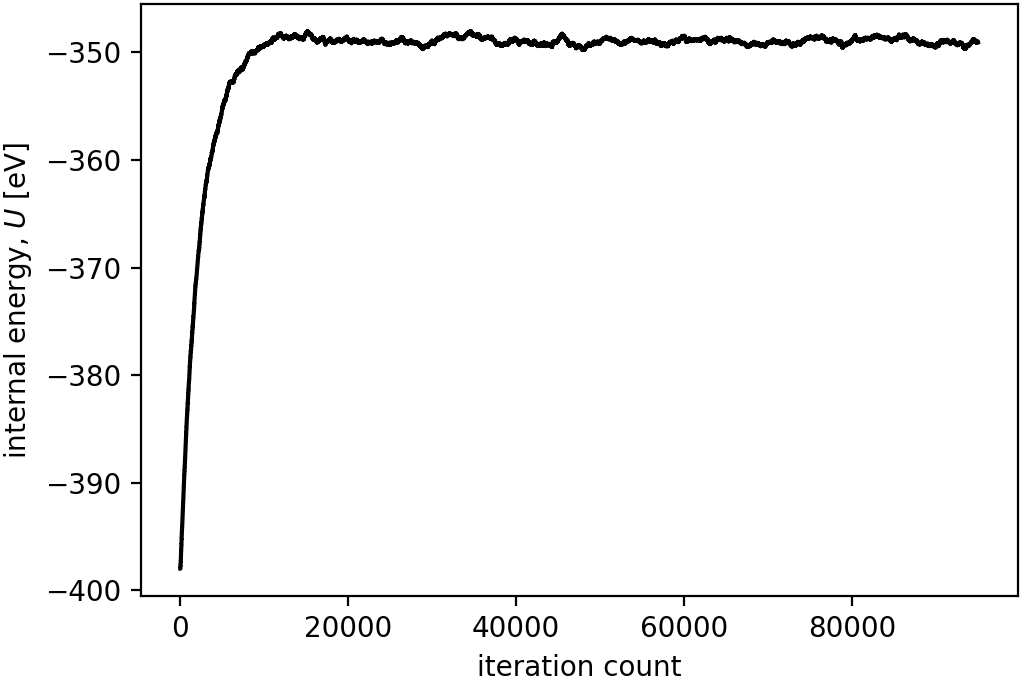
\includegraphics[width=0.49\textwidth]{Figures/swap_any_two_convergence.png}
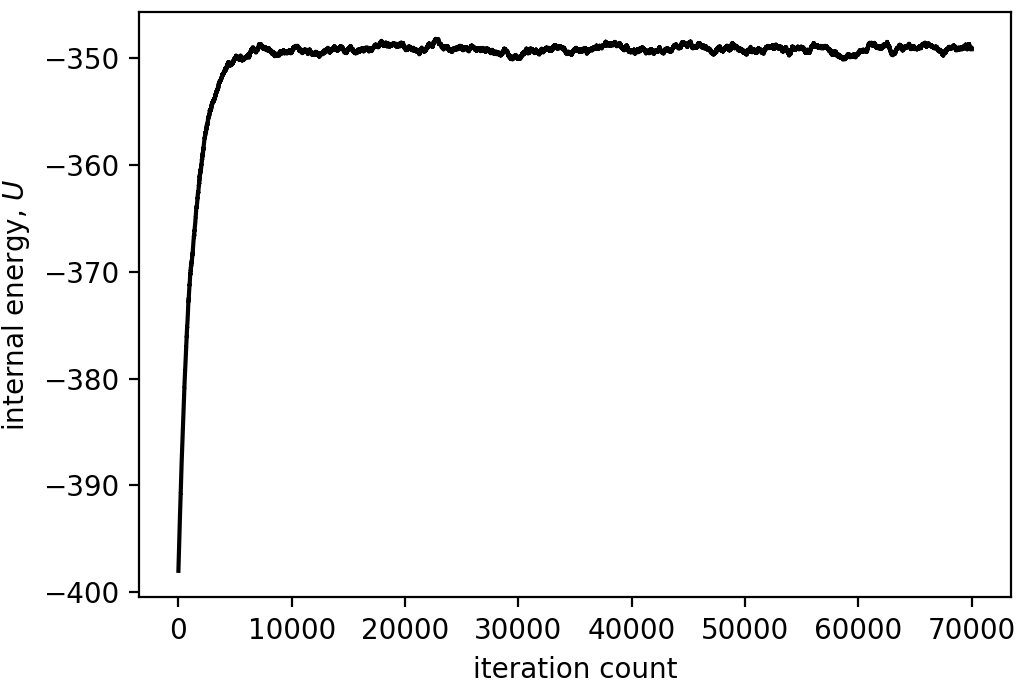
\includegraphics[width=0.49\textwidth]{Figures/swap_A_B_only_convergence.png}
\caption{Internal energy versus iteration with $L=100$, $d=2$, $x=0.5$, $\beta=0.1$, $w_{AA}=w_{AB}=-10 \times 10^{-3},w_{BB} = -30 \times 10^{-3}$ eV; both simulations were run until the percentage error in the mean energy was less than 0.005\%.
The left figure is when swaps may exchange any two sites (independent of their types), while the right figure permits exchanges only between A and B sites.}
\label{fig:swap}
\end{figure}


\newpage
\bibliography{references.bib}
References (USE BIBTEX THOUGH)


\end{document}

